\section{The Hj and Hjj taggers}\label{sec:HjHjjtaggers}
In this section we describe discriminators aiming at identifying jets that originate from a Higgs decaying to two Ws.
In particular, we target the 2lss category in which the ttH signal decays, in the highest fraction of events, according to the following chain:
$$(t) (t) (H) \rightarrow  (bW) (bW) (WW^*) \rightarrow (bjj)  (b\ell\nu_{\ell}) (\ell\nu_{\ell}jj)$$
We therefore expect 2 b quark jets, 4 jets, 2 same-sign leptons, and missing energy in the final state,
altough, in order to increase the signal acceptance, the analysis requires the presence of at least 4 jets overall.
This means that the Higgs jets do not necessarily enter the signal region.

In order to deal with both the complicated jet combinatoric and the possibility that not all the jets originating from Higgs are selected,
two discriminators are developed: the Higgs-jet (Hj) tagger and the Higgs-dijet (Hjj) tagger.
The Hj tagger is an object discriminator that exploits jet identification and kinematic properties
in order to assess the likelihood of a jet of originating in the decay $H \rightarrow WW^* \rightarrow \ell\nu_{\ell}jj$.
The Hjj tagger is a discriminator that considers geometric and kinematic features in order to estimate the 
likelihood of a jet pair originating again from $H \rightarrow WW^* \rightarrow \ell\nu_{\ell}jj$.

The discriminators are developed considering the BDT  multivariate technique.
We rely on the powheg ttH signal samples to define both the signal and the background in the training.
For the Hj (Hjj) tagger the signal is represented by reconstructed jets (dijet pair) that are (is) matched at gen-level to jets (dijet pair)
of the process $H \rightarrow WW^* \rightarrow \ell\nu_{\ell}jj$, while the background is given by the other reconstructed jets (dijet pairs)
in the same event. 
For the training, we consider the phase space of events that enter the 2lss, where leptons are muons, selection with 0 $\tau_h$.

In the following subsections we list the variables used for the Hj and Hjj taggers and their expected BDT distributions.

\subsection{Hj variables and performances}
The variables used for the Hj tagger are:
\begin{itemize}
\item minimum dR of the jet and one of the lepton
\item maximum dR of the jet and one of the lepton
\item jet pT
\item jet b-tagging discriminator
\item jet quark-gluon discriminator
\end{itemize}

The performances of the Hj tagger are illustrated in Fig. \ref{fig:HjDistrROC}.

\begin{figure}[htb]
 \centering
   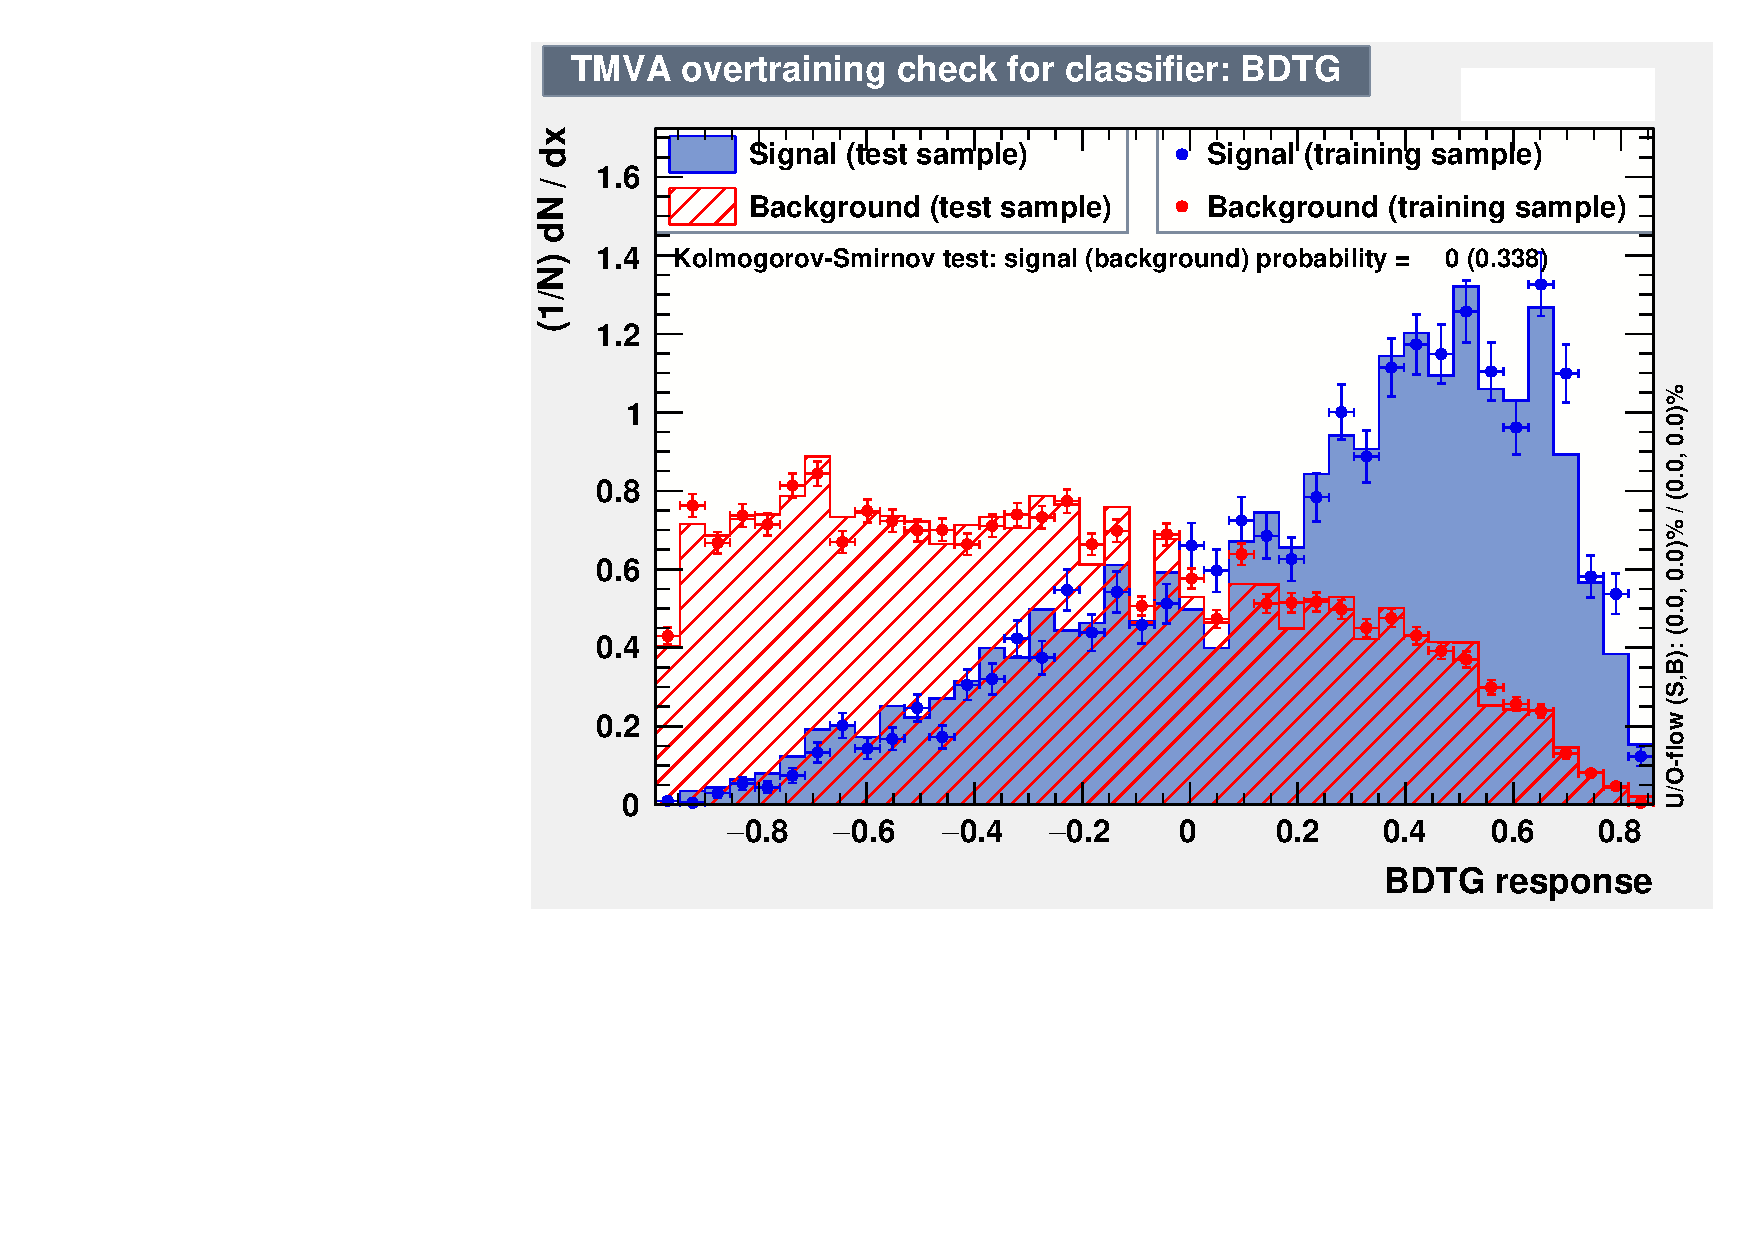
\includegraphics[width=0.48\textwidth]{plots_HjHjj/Jtagger_Ks.pdf}
   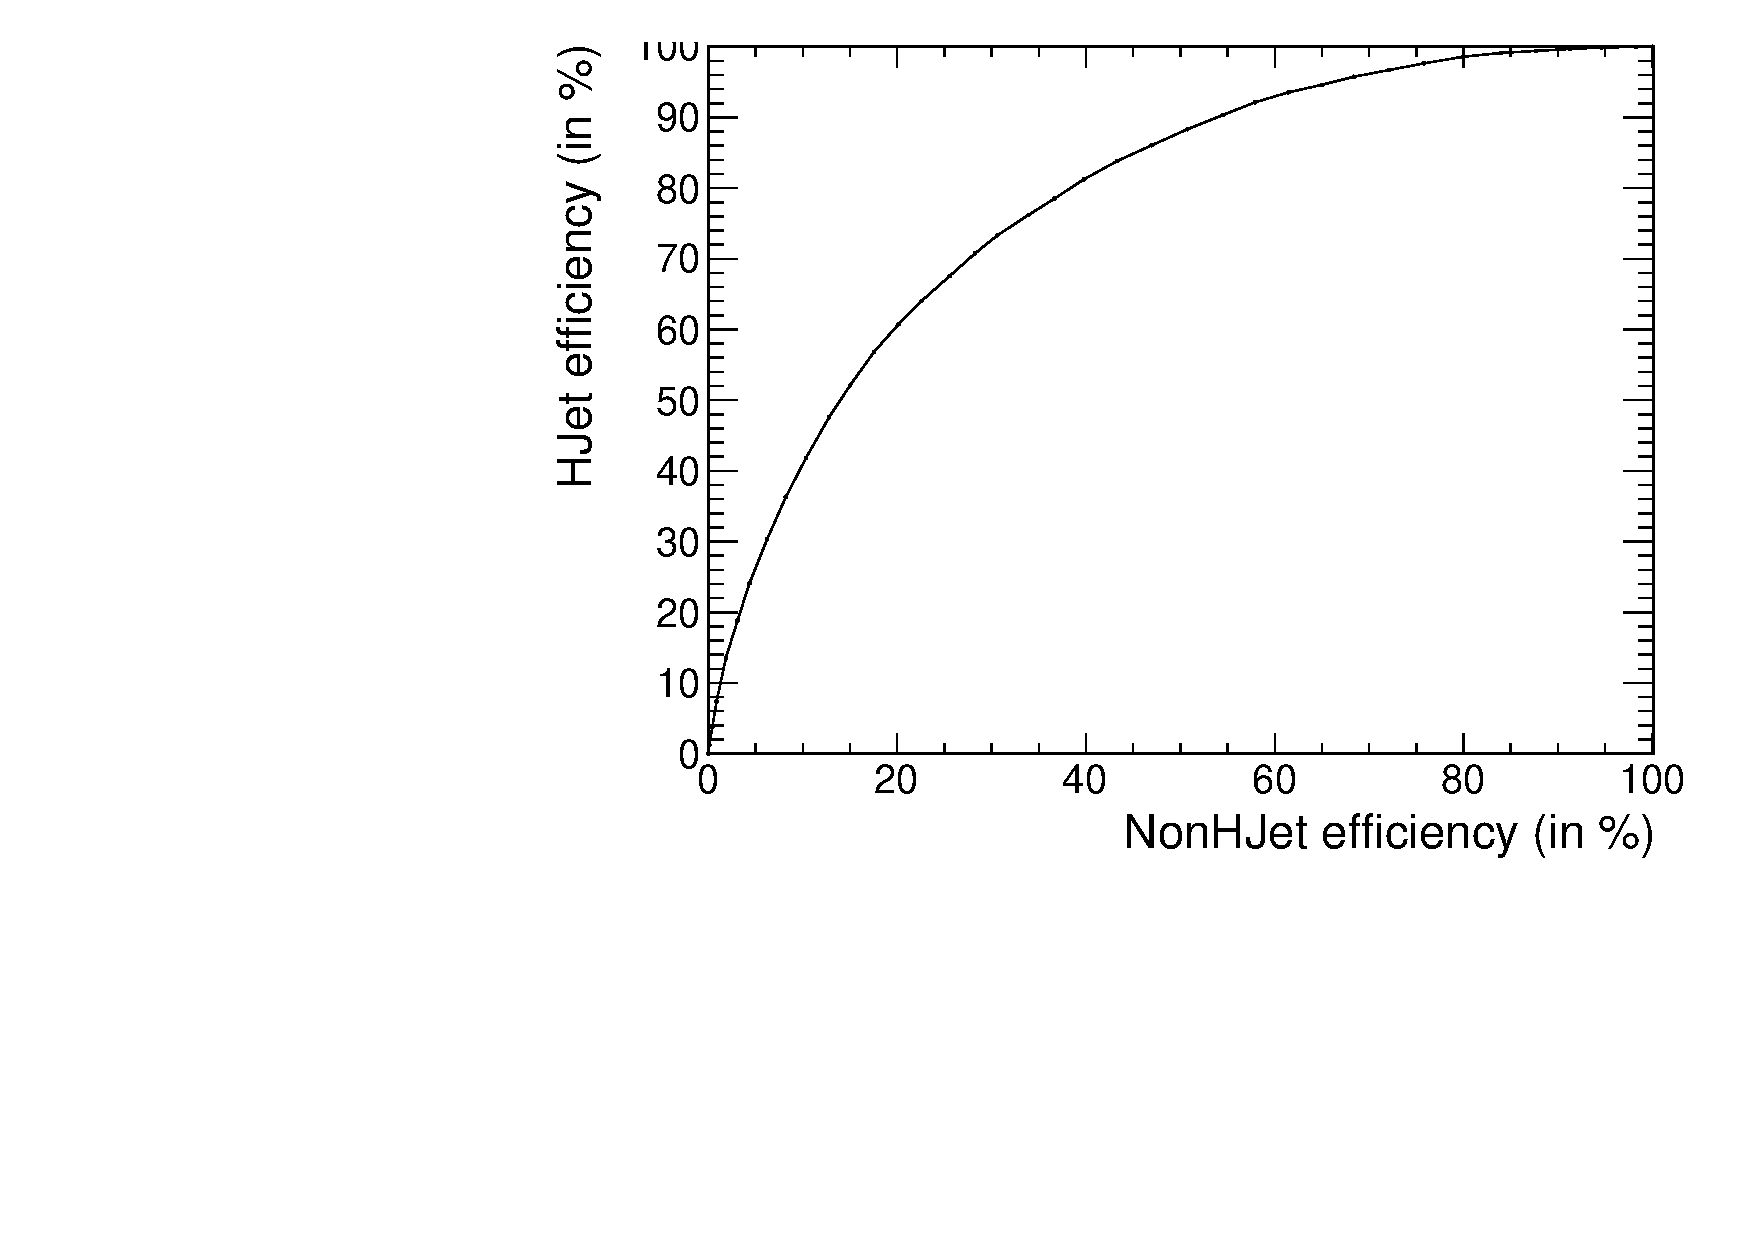
\includegraphics[width=0.48\textwidth]{plots_HjHjj/JetTagger_DiMuSR.pdf}
   \caption{The Hj distribution (left) and ROC (right). Signal and background composition are described in the text.}
  \label{fig:HjDistrROC}
\end{figure}


\subsection{Hjj variables and performances}
The variables used for the Hj tagger are:
\begin{itemize}
\item sum of the Hj taggers for the two jets 
\item dR of the two jets
\item minimum dR between the jet pair and another jet
\item ratio of the minimum and maximum dR between the jet pair and another jet
\item dijet mass
\item mass of the dijet plus the closest lepton
\end{itemize}

The performances of the Hjj tagger are illustrated in Fig. \ref{fig:HjjDistrROC}.

\begin{figure}[htb]
 \centering
   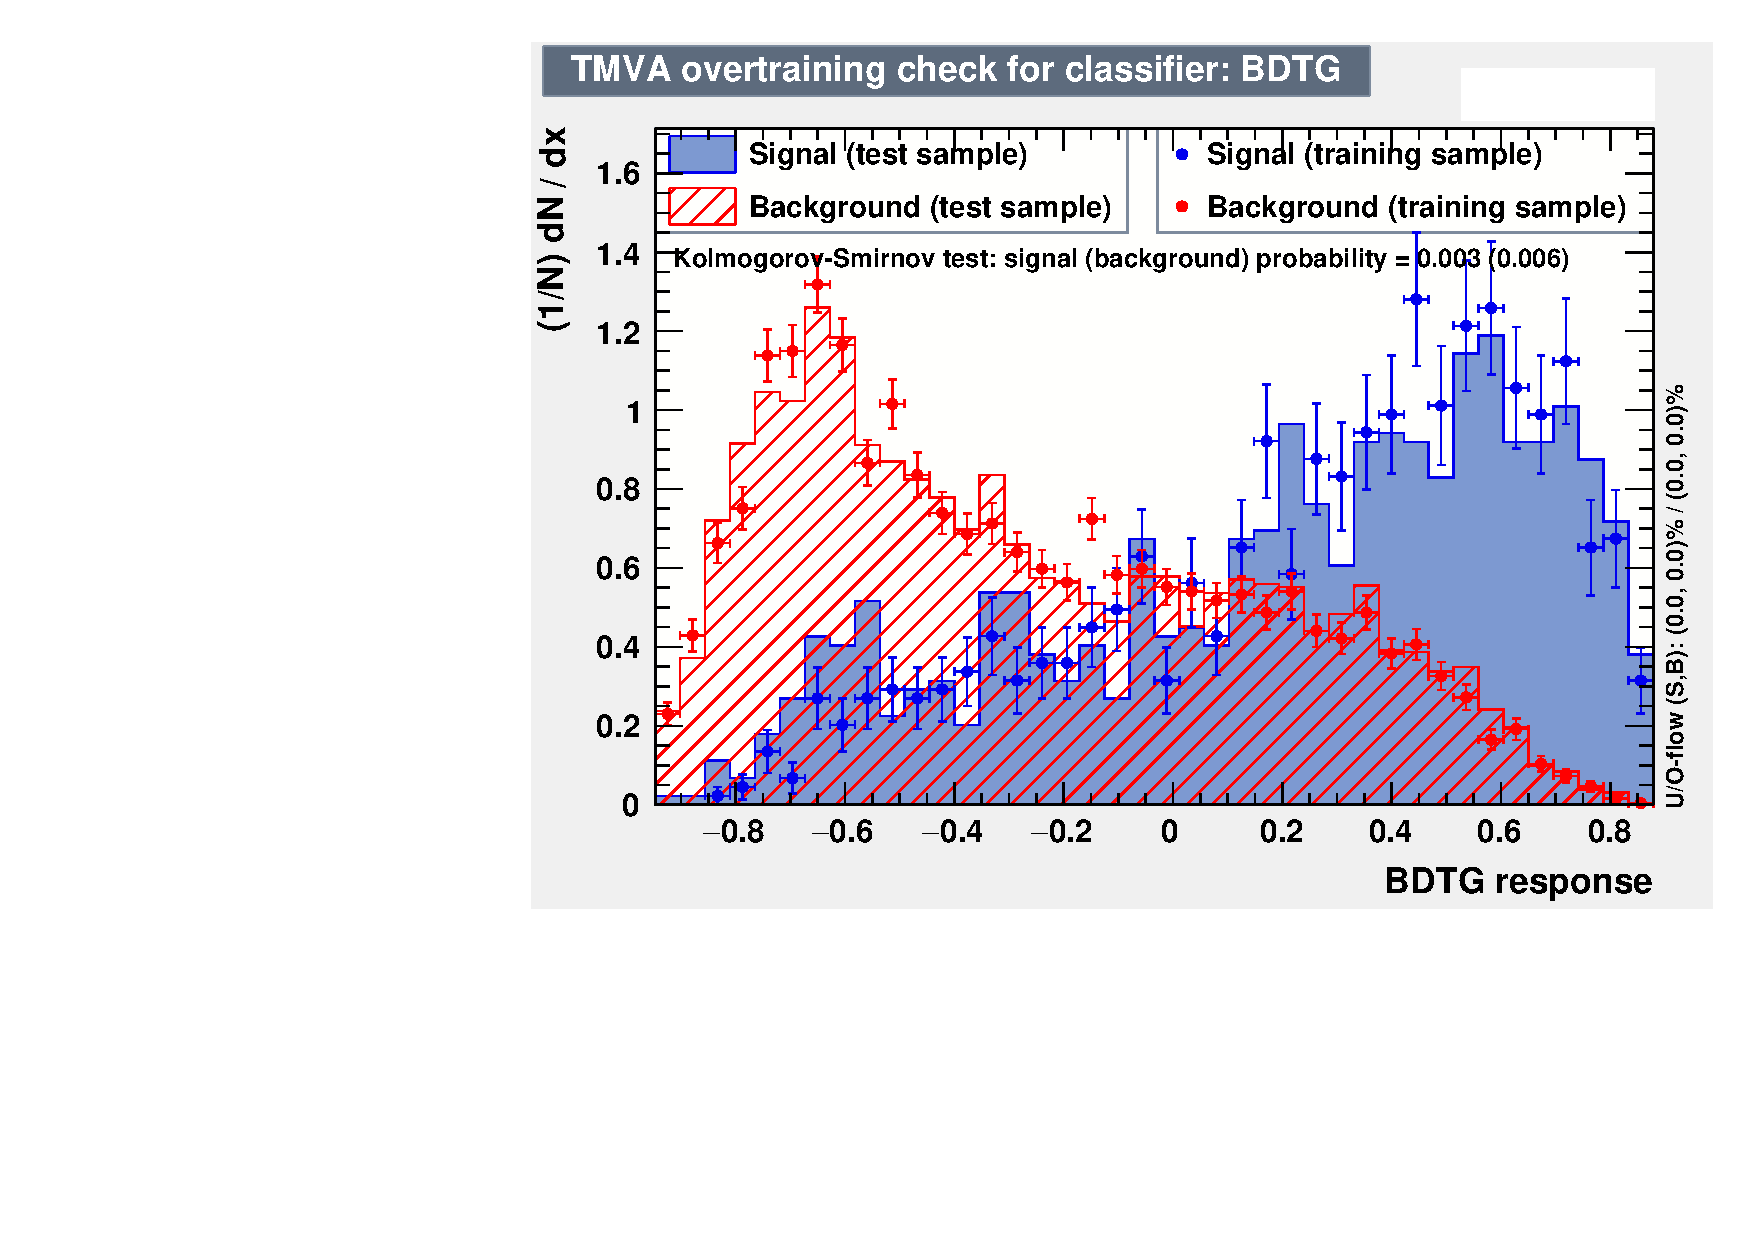
\includegraphics[width=0.48\textwidth]{plots_HjHjj/JJtagger_Ks.pdf}
   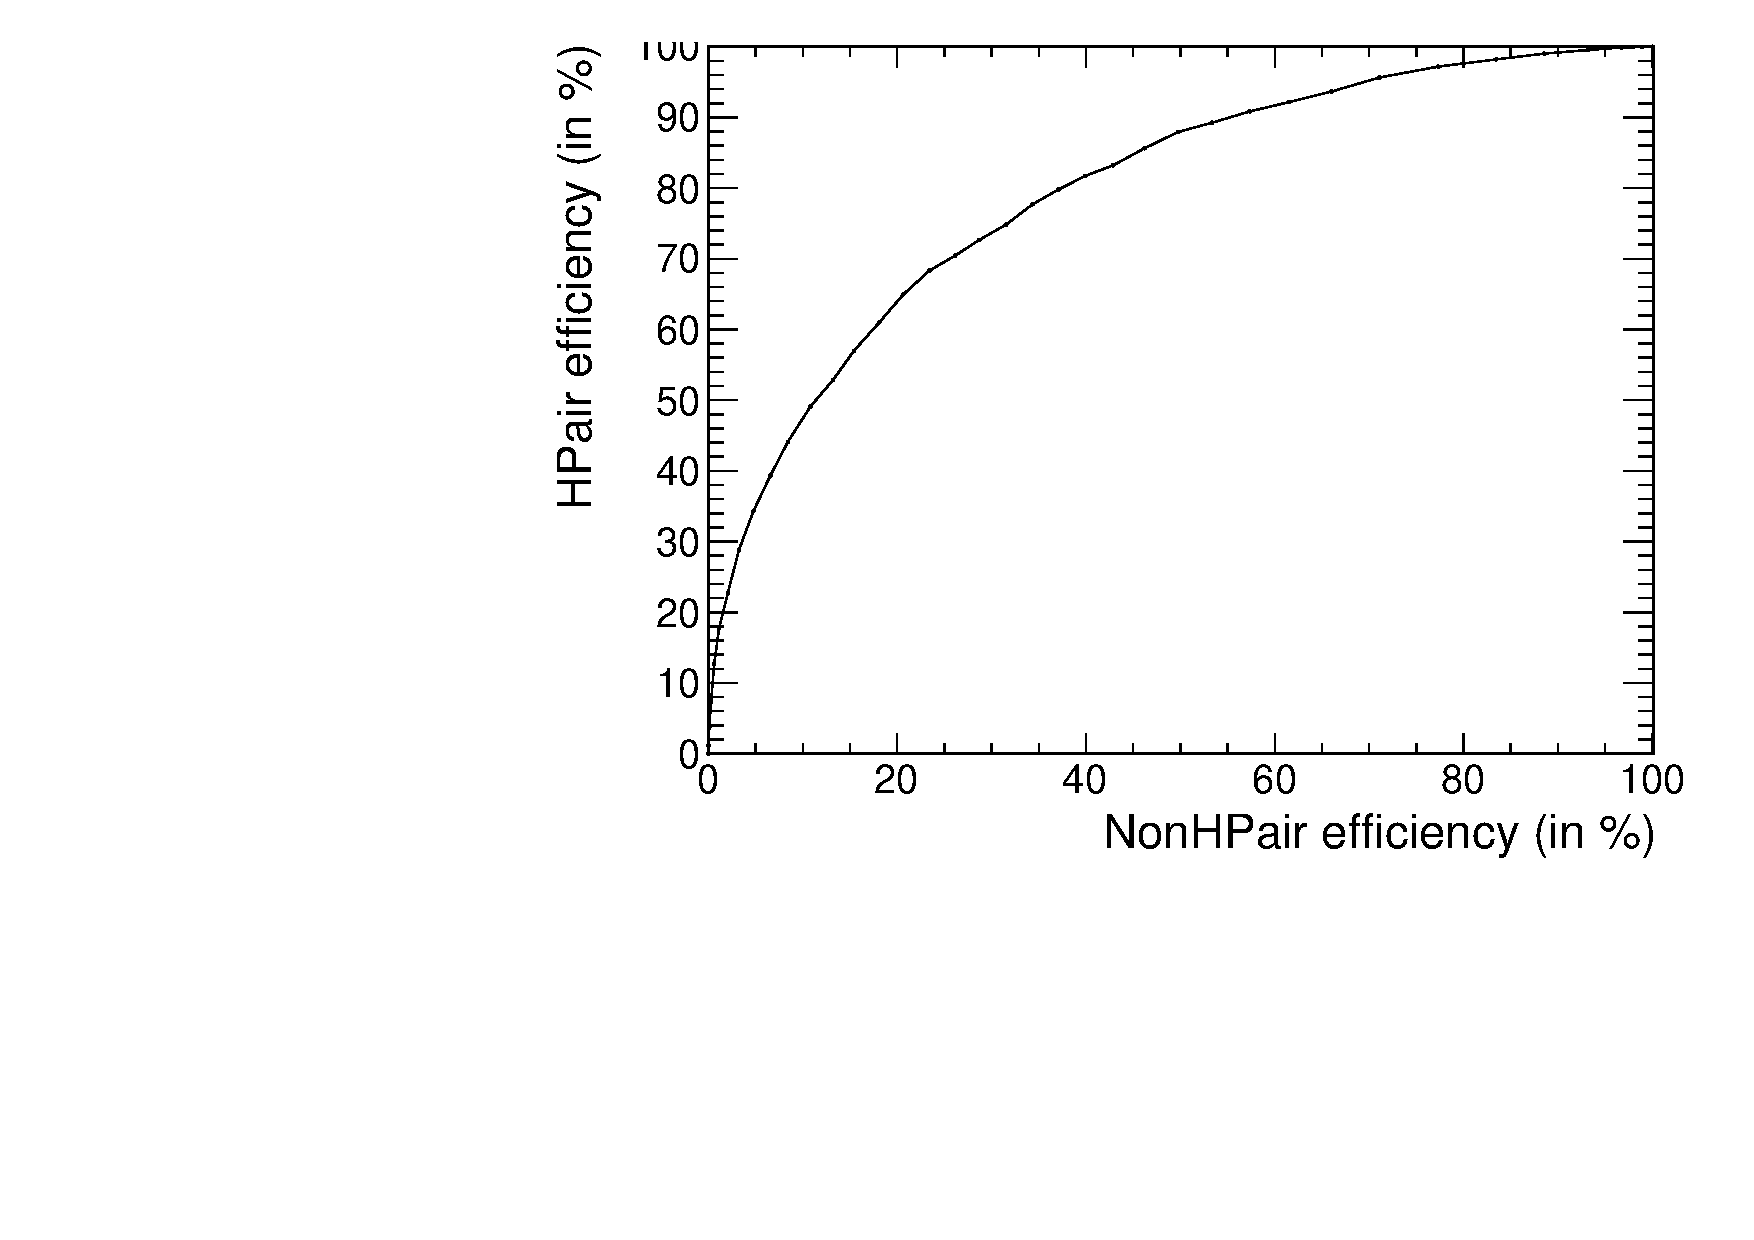
\includegraphics[width=0.48\textwidth]{plots_HjHjj/JetPair_30Jan.pdf}
   \caption{The Hjj distribution (left) and ROC (right). Signal and background composition are described in the text.}
  \label{fig:HjjDistrROC}
\end{figure}
